\documentclass{beamer}
%\usetheme{metropolis}
\usepackage[utf8]{inputenc}
\usepackage{xcolor}
\usepackage{tikz}



%Information to be included in the title page:
\title{Bayesian Statistics - Homework 2}
\subtitle{Gabry et al., \textit{Visualization in Bayesian workflow} (2018)}
\author{Roberto Corti}
\date{\today}

\setbeamercolor{background canvas}{bg=white}

\begin{document}
	
	\frame{\titlepage}
	
	\begin{frame}{Visualization in Bayesian workflow}{A pipeline for our work}
		Visualization is an invaluable way of justifying and criticize a statistical model.\\
		\vspace{0.5cm}
		Phases of statistical workflow:
		\begin{itemize}
			\item Set up an initial model
			\item Model check
			\item Computational checks for the inference algorithm 
			\item Posterior predictive checks
			\item Model comparison
		\end{itemize} 
	\vspace{0.5cm}
	
	\textbf{Example}: Estimate global $\text{PM}_{2.5}$ concentration
	\end{frame}
	

	\begin{frame}{Exploratory data analysis}{More than just plotting the data}	
		\only<1>{
		\begin{center}
			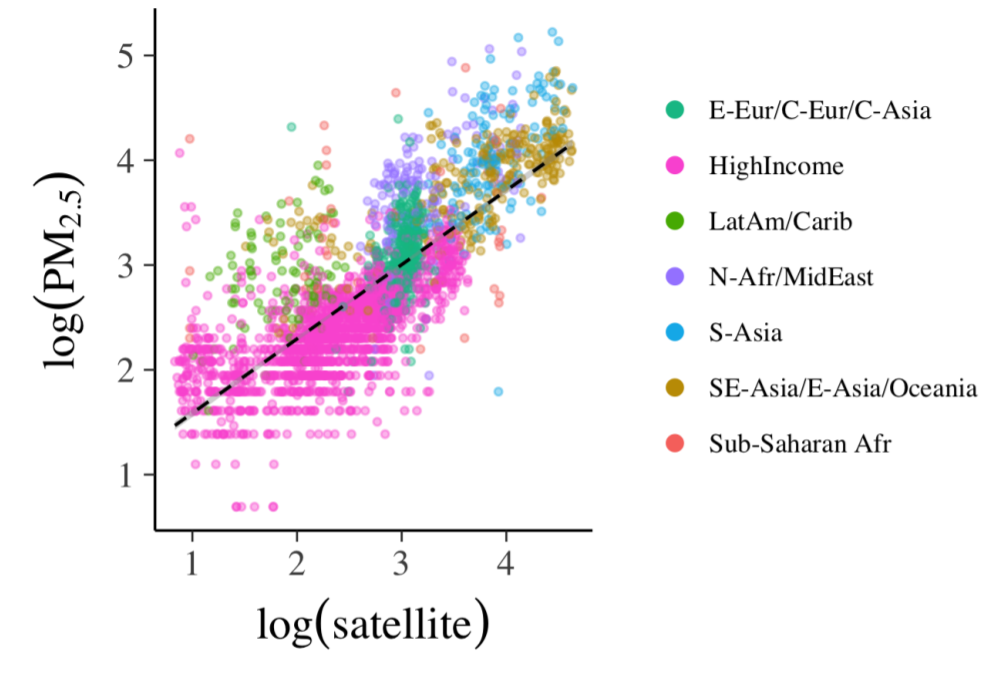
\includegraphics[scale=0.4]{images/model1.png}
		\end{center}
		}
	
		\only<2>{
			
		\begin{center}
			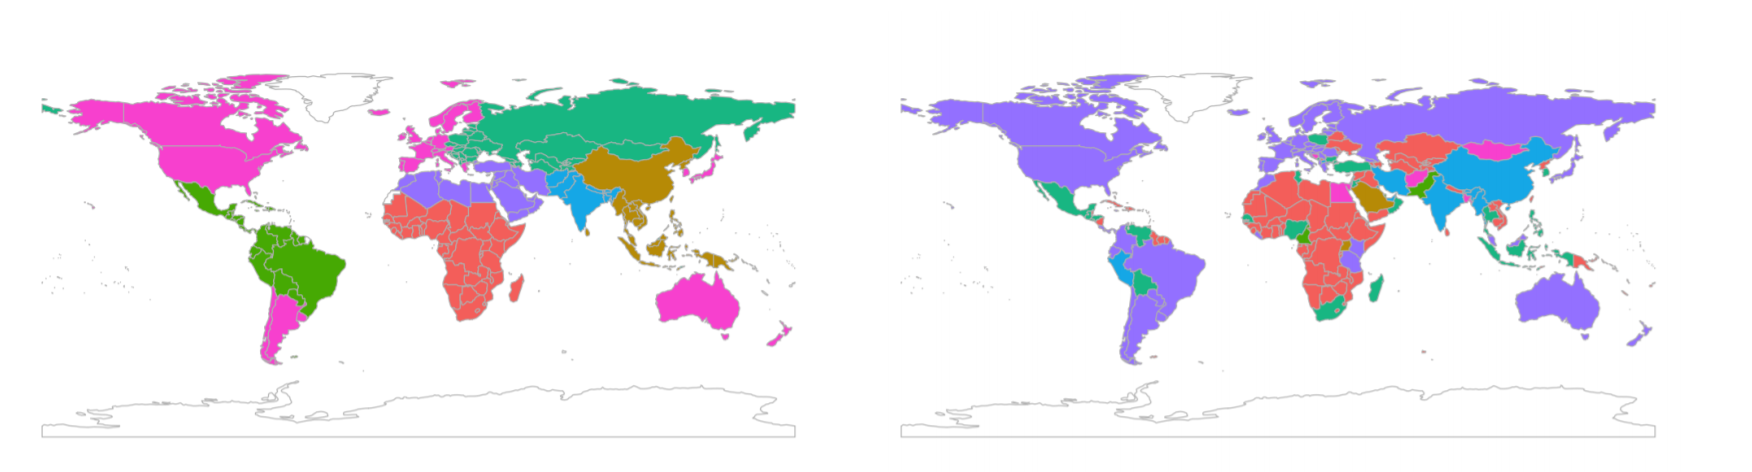
\includegraphics[scale=0.3]{images/regions.png}
		\end{center}
	
		\begin{figure}
			\centering
			\begin{minipage}{.5\textwidth}
				\centering
				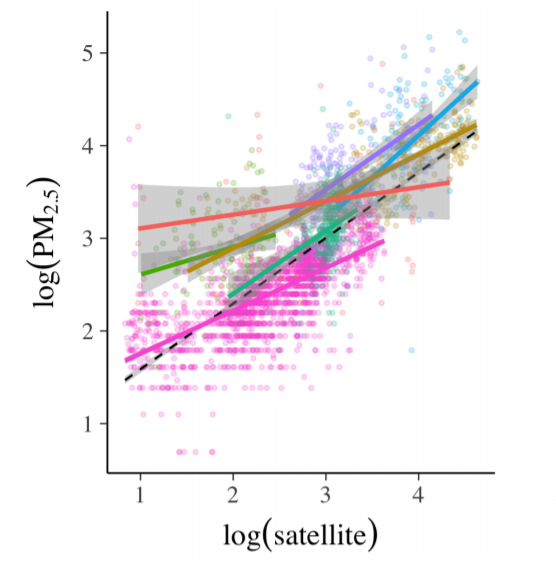
\includegraphics[width=.75\linewidth]{images/model2.png}
			\end{minipage}%
			\begin{minipage}{.5\textwidth}
				\centering
				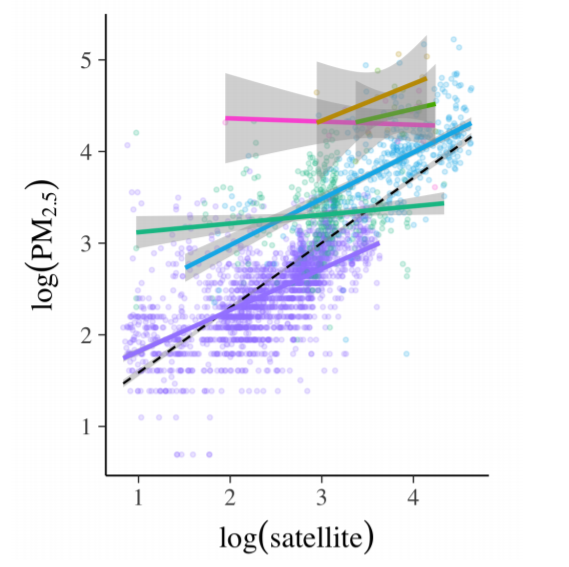
\includegraphics[width=.75\linewidth]{images/model3.png}
			\end{minipage}
		\end{figure}
		}
	
		\only<3>{
		\begin{itemize}
			\item \textbf{Model 1}: simple linear regression,
			\vspace{0.6cm}
			\item \textbf{Model 2}: multilevel model where 			observations are stratified by WHO super-regions,
			\vspace{0.6cm}
			\item \textbf{Model 3}:  multilevel model where
			observations are stratified by clustered super-region.
		\end{itemize}
		
			}
	\end{frame}

	\begin{frame}{Prior predictive checking}{Fake data can be almost as valuable as real data}
		\textbf{Generative model}:	$ \theta^* \sim p(\theta) \longrightarrow y^* \sim p(y|\theta^*) \Longleftrightarrow  y^* \sim p(y)$
		
		\begin{figure}
			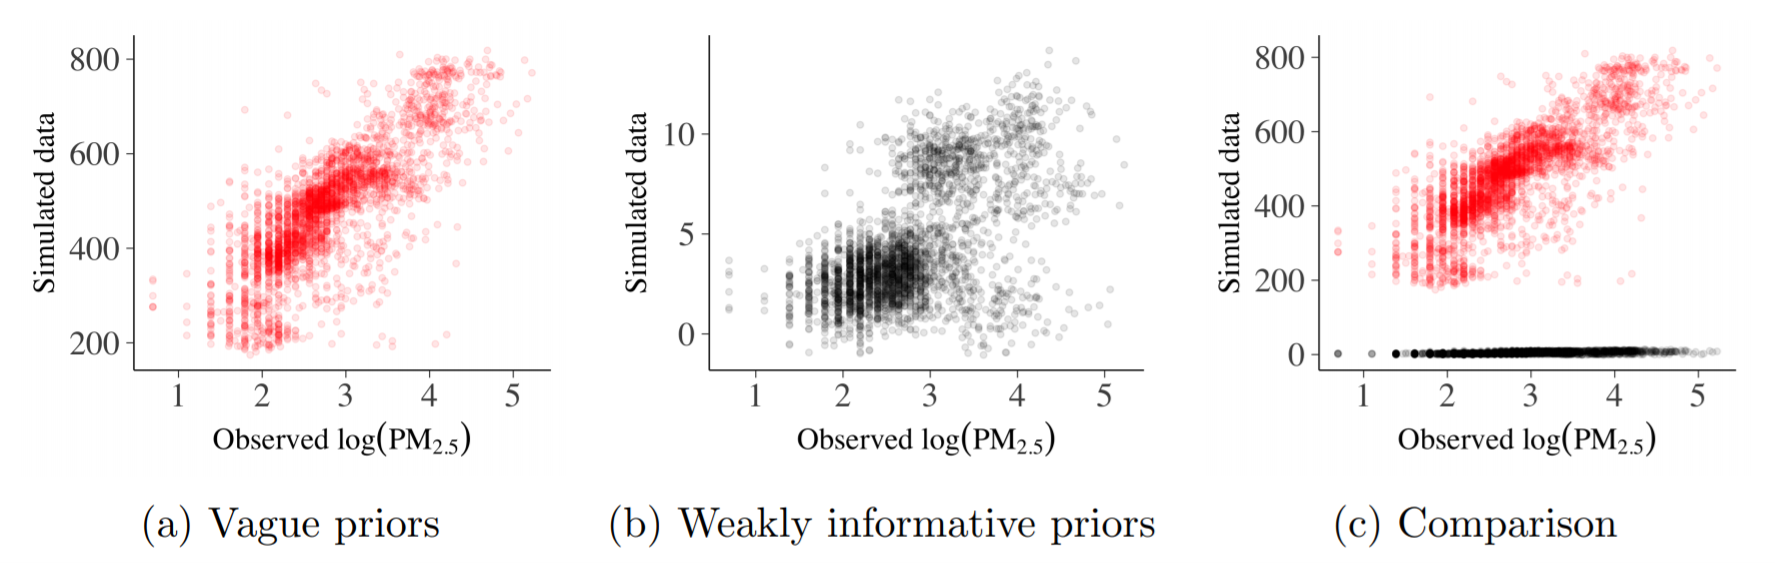
\includegraphics[scale=0.3]{images/fake_data.png}
		\end{figure}
			
		
		
	\end{frame}

	\begin{frame}{MCMC diagnostics}{Moving beyond trace plots}
		
			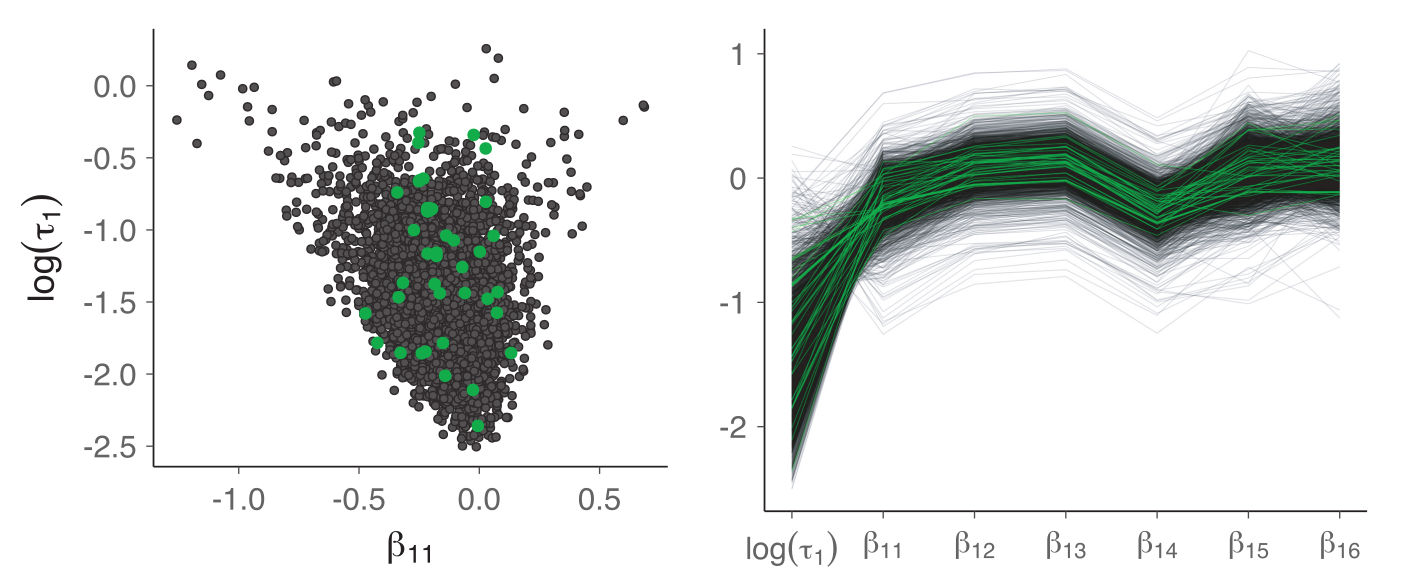
\includegraphics[scale=0.23]{images/scatterplot.png}
		
	\end{frame}
	
	\begin{frame}{Posterior predictive checks}{How did we do?}
		\textbf{Posterior predictive distribution}: $p(\widetilde{y}| y) = \int d\theta ~ p(\widetilde{y}|\theta) p(\theta | y)$
		
		\only<1>{
			\begin{figure}
				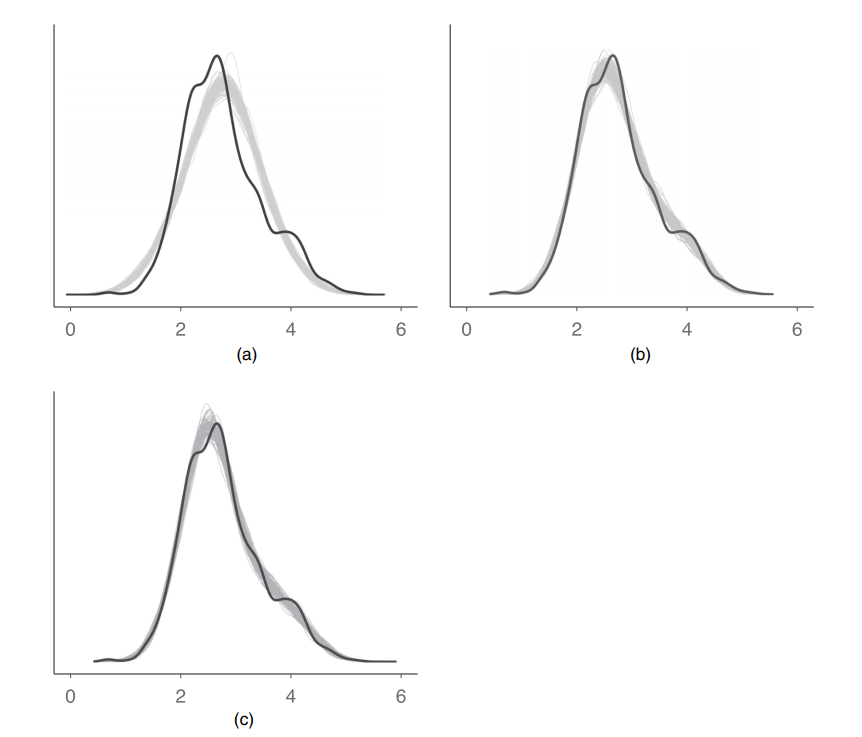
\includegraphics[scale=0.4]{images/posterior_predictive.png}
			\end{figure}
		}
	
		\only<2>{
			\begin{figure}
				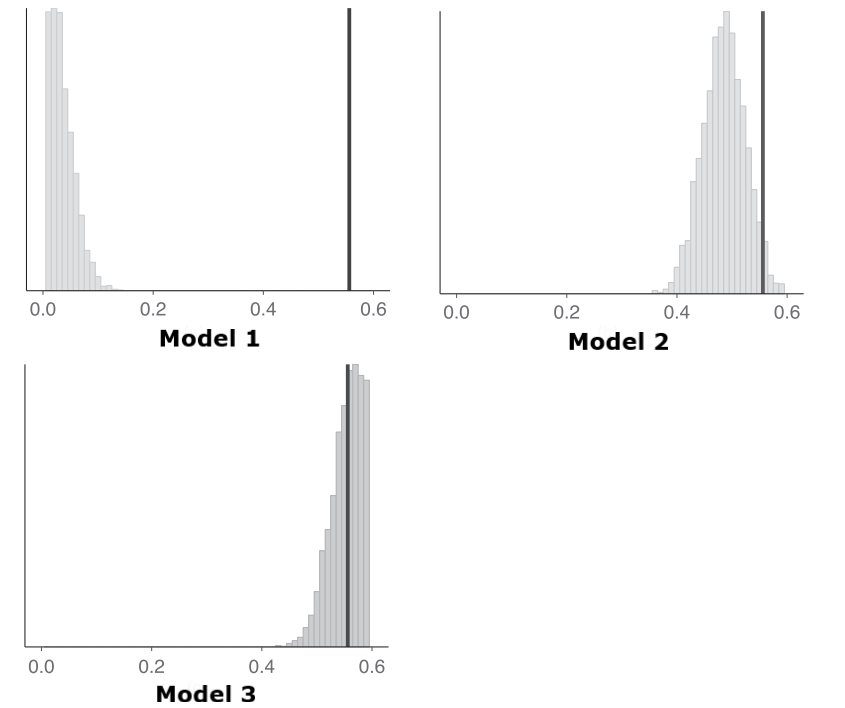
\includegraphics[scale=0.42]{images/skew.png}
			\end{figure}
		}
		
	\end{frame}

	\begin{frame}{Model comparison}{Looking \textit{when} and \textit{where} a model is better than another}
		\textbf{LOO predictive distrubution}: $p(y_i | y_{-i}) $
		
		\begin{figure}
			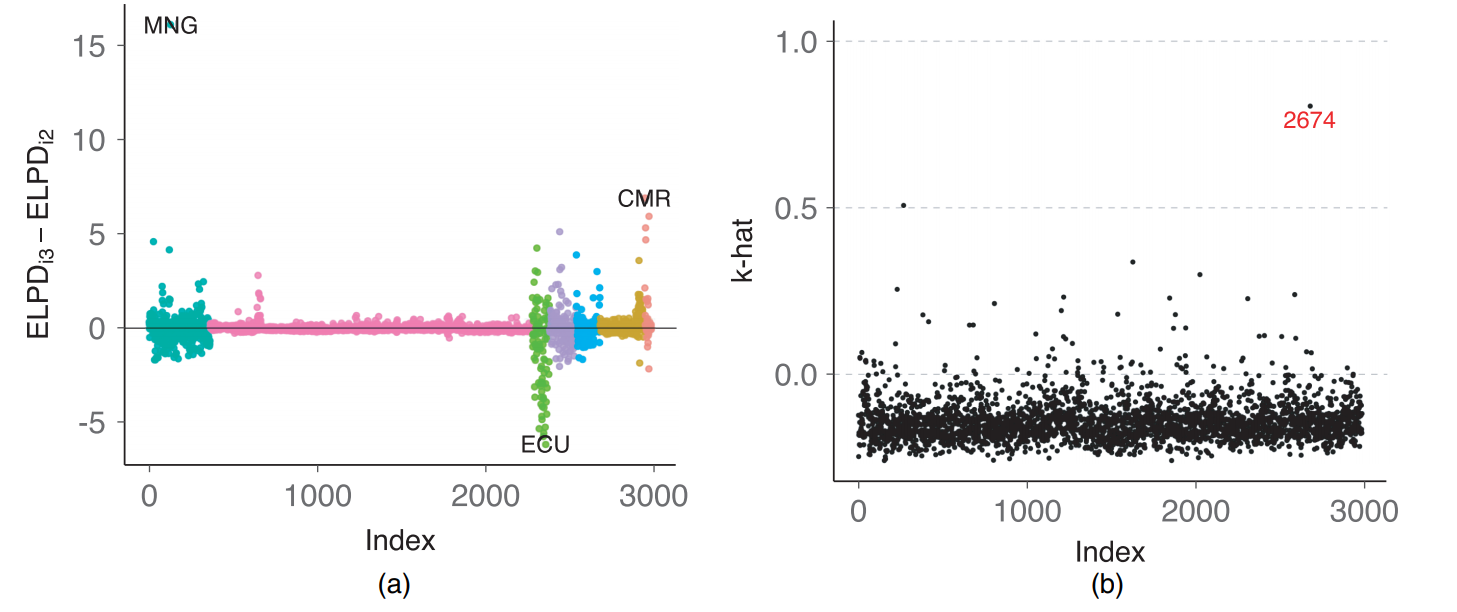
\includegraphics[scale=0.36]{images/model_comparison.png}
		\end{figure}
		
	\end{frame}



	
\end{document}